\documentclass[10pt]{beamer}

\usetheme{metropolis}
\usepackage{appendixnumberbeamer}

\usepackage{booktabs}
\usepackage[scale=2]{ccicons}

\usepackage{pgfplots}
\usepgfplotslibrary{dateplot}

\usepackage{xspace}
\newcommand{\themename}{\textbf{\textsc{metropolis}}\xspace}

\usepackage{bm}

\title{Markov Decision Process in Dynamic Optimization of Fare Price}
\subtitle{ROBUST 2016}
\date{September 15, 2016}
\author{Jan Kislinger}
\institute{Department of Probability and Mathematical Statistics, Charles University}

\begin{document}

\maketitle

%--------------------------------------------------------------------
\begin{frame}[fragile]{Decision-dependent Newsboy Problem}

	\begin{itemize}
		\item Number of demanded newspapers $D$
		\item Fixed inventory level $n$
		\item Price $p$ as a decision variable
			\[
				\pi_k (p) = \mathbb{P} [D = k \vert p ]
			\]
		\item Objective: maximize expected return wrt. price
			\[
				\mathbb{E} [p D] = p \left( \sum_{k=0}^{n} k \pi_k (p) + n \sum_{k=n+1}^{\infty} \pi_k (p) \right)
			\]
		\item
			E.g. Poisson demand with log-linear model
			\[
				\pi_k (p) = \frac{\lambda^k (p)}{k!} \textrm{e}^{-\lambda(p)}, \qquad
				\lambda^k (p) = \textrm{exp} (\beta_0 + \beta_1 \textrm{log} (p))
			\]

	\end{itemize}
		
\end{frame}

%--------------------------------------------------------------------
\begin{frame}[fragile]{Optimal control}
  
	\begin{itemize}
		\item Selling over time interval $D_t, t \in [0,1]$
		\item Markov chain with state space representing number of sold newspapers
			\[
				\mathcal{S} = \left\{ 0, ..., n \right\}, \qquad X_0 = 0
			\]
		\item Objective: find optimal policy $\varphi^*$ for price
			\[
				\varphi: \mathcal{S} \times [0,1] \to \mathbb{R}^+
			\]
		\item Piecewise deterministic function
	\end{itemize}
	
\end{frame}

%--------------------------------------------------------------------
\begin{frame}[fragile]{Random inventory level}
  
	\begin{itemize}
		\item Model for train fare price with $K$ stations
		\item Single passenger type, single class
		\item $\binom{K}{2}$ routes indexed by boarding and exiting stations $(k,l)$, $1 \leq k < l \leq K$
		\item Bounded sums of inventory levels
			\[
				\mathcal{S} = \left\{ \bm{s} \in \mathbb{N}_0^{\binom{K}{2}}: \sum_{k=1}^h \sum_{l=h+1}^K s_{k,l} \leq n, 1 \leq h \leq K-1 \right\}
			\]
		\item Non-computable transition probabilities
	\end{itemize}

\end{frame}

%--------------------------------------------------------------------
\begin{frame}[fragile]{Simulated optimization I}

  \begin{center}
		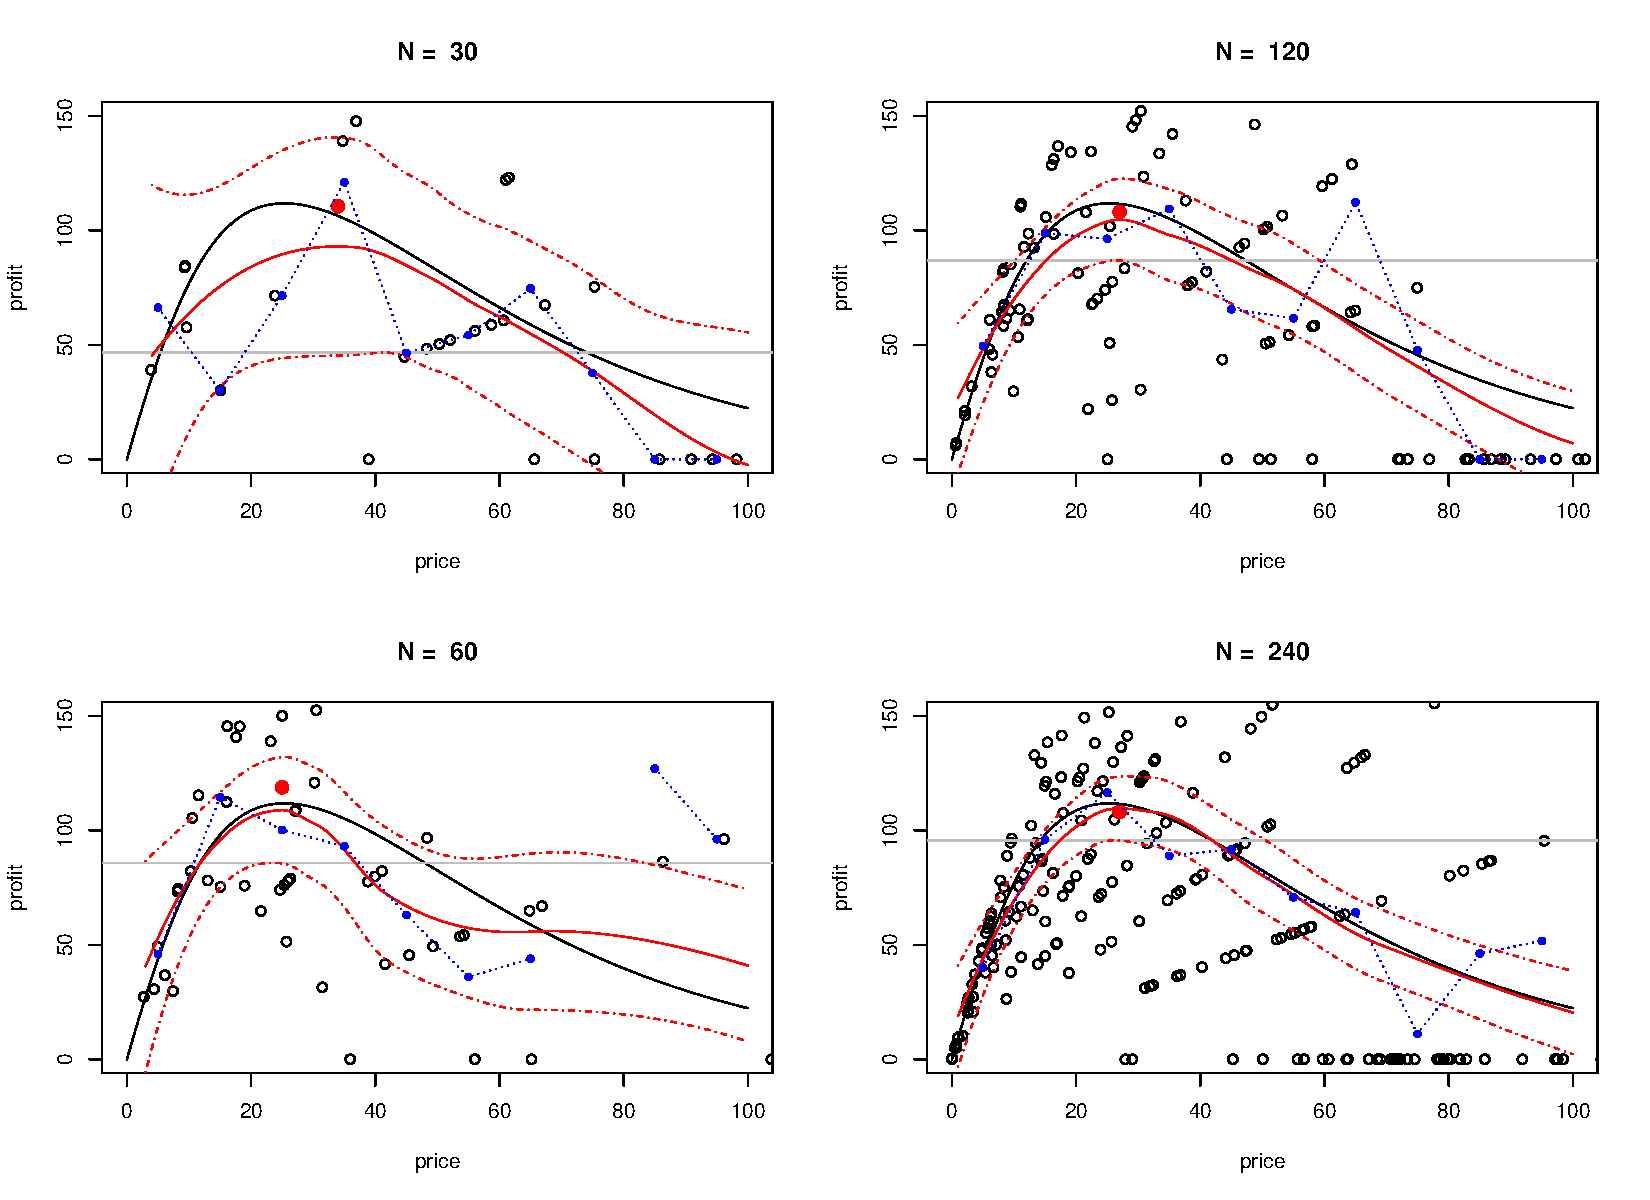
\includegraphics[width=\textwidth]{figures/newsboy_old.pdf}
	\end{center}
	
\end{frame}

%--------------------------------------------------------------------
\begin{frame}[fragile]{Simulated optimization II}
	
	\begin{center}
		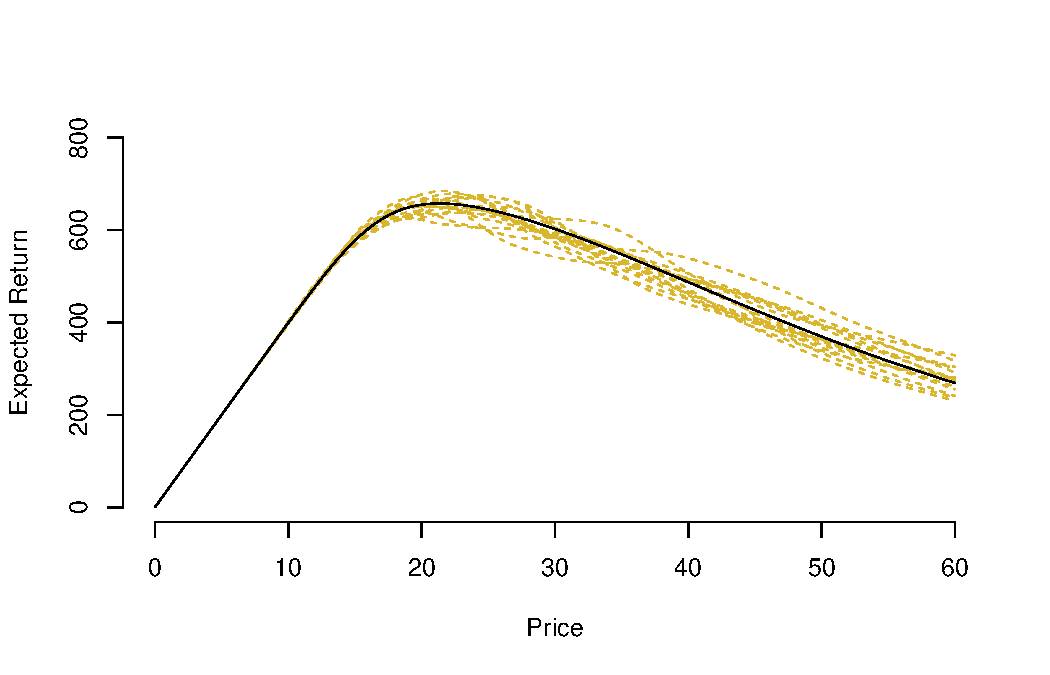
\includegraphics[width=\textwidth]{figures/newsboy.pdf}
	\end{center}
\end{frame}

%--------------------------------------------------------------------
\begin{frame}[fragile]{Further generalizations}
  
	\begin{itemize}
		\item Multiple passenger types
		\item Unlimited number of passenger per ticket
		\item Multiple seat classes (substitutes)
		\item Distinct seats, passenger can choose a seat
	\end{itemize}

\end{frame}

%--------------------------------------------------------------------
\begin{frame}[fragile]{Content of the Poster}
  
	\begin{itemize}
		\item Formal notation of objects and optimization problem
		\item Model for transition intensities (demand)
		\item Algorithms for simulated optimization
		\item Way how to transform the problem to endogenous
		\item Numerical results for fictional train
	\end{itemize}

\end{frame}

\begin{frame}[standout]
  Thank You for Your Attention!
\end{frame}



\end{document}
